\documentclass[12pt]{article}
\usepackage[top=2in, bottom=1.5in, left=1in, right=1in]{geometry}
\usepackage{pdfpages}
\usepackage{fancyhdr}
\usepackage{pgfplots}
\usepackage{hyperref}
\usepackage[T1]{fontenc}
\usepackage{graphicx}
\graphicspath{ {images/} }
\pagestyle{fancy}
\fancyhf{}
\fancyhead[LE,RO]{NETWORK RELIABILITY API FOR FIREFOX OS}
\fancyfoot[CE,CO]{\leftmark}
\fancyfoot[LE,RO]{\thepage}

\begin{document}
\title{NETWORK RELIABILITY API FOR FIREFOX OS\\Improving Efficiency Through Analysis of Network Metadata}
\maketitle
\begin{center}
    \author{John Zeller\\Pok Yan Tjiam\\Jonathan McNeil}
\end{center}
\pagebreak

\tableofcontents
\pagebreak

\section{Introduction}
% Who requested it?
% Why was it requested?
% What is its importance?
% Who was/were your client(s)?
% Who are the members of your team?
% What were their roles?
% What was the role of the client(s)? (I.e., did they supervise only, or did they participate in doing development)

This project was requested by Mozilla, specifically the team working on Firefox OS. Our customer during the course of our project was Dietrich Ayala, a Project Manager working on Firefox OS and a member of the Mozilla family since February 2006. Dietrich's role in our project took many forms, and evolved as what we needed did so. Initially, he helped on board us to the Firefox OS platform, providing us with plenty of documentation to wrap our heads around, and once we have devoured this information, he was quick to setup meeting with members form the Firefox OS networking team. Throughout the year Dietrich was always available via IRC, Skype, Email, and Cell, whenever we needed him. And if he could not answer a question for us, he knew who could.
\\\\
The members of our team were John Zeller, Pok Yan Tjiam, and Jonathan McNeil. John Zeller, having worked with Mozilla for over a year as an intern and contractor, acted as a de facto team lead during the course of the project. Pok Yan Tjiam worked on \_\_\_. Jonathan McNeil worked on \_\_\_.
\\\\
The purpose of this project was to help work towards giving developers a tool that allows them to avoid the typical environment agnostic network request paradigm. As it currently stands, most developers create apps with little to no information about the quality of the network. In their apps, they typically run network requests in a dumb loop, which simply tries continually until the request succeeds. This is wasteful in terms of both battery and data, and overloads an often times already overloaded network.
\\\\
Firefox OS is not a direct competitor to the well known giants in the mobile OS space, but is aimed at being a good solution for the next 4 billion people coming online; the majority of which are coming online in developing countries where network infrastructure is literally decades behind, having a profoundly negative impact on user experience. In many cases poor network conditions can even render some applications non-functional. Aside from out-dated networks, some areas of these developing countries also have unreliable electrical grids, which can make charging a phone take days for many users living with the most unreliable grids. And this problem is only growing worse, at an ever growing pace. In the next 30 days, India alone is expected to account for 5 million new internet users.
\pagebreak

\section{Requirements Document}
\subsection{Original}
Here is our original requirements document, featuring the details of our project as we understood them at the time it was written.
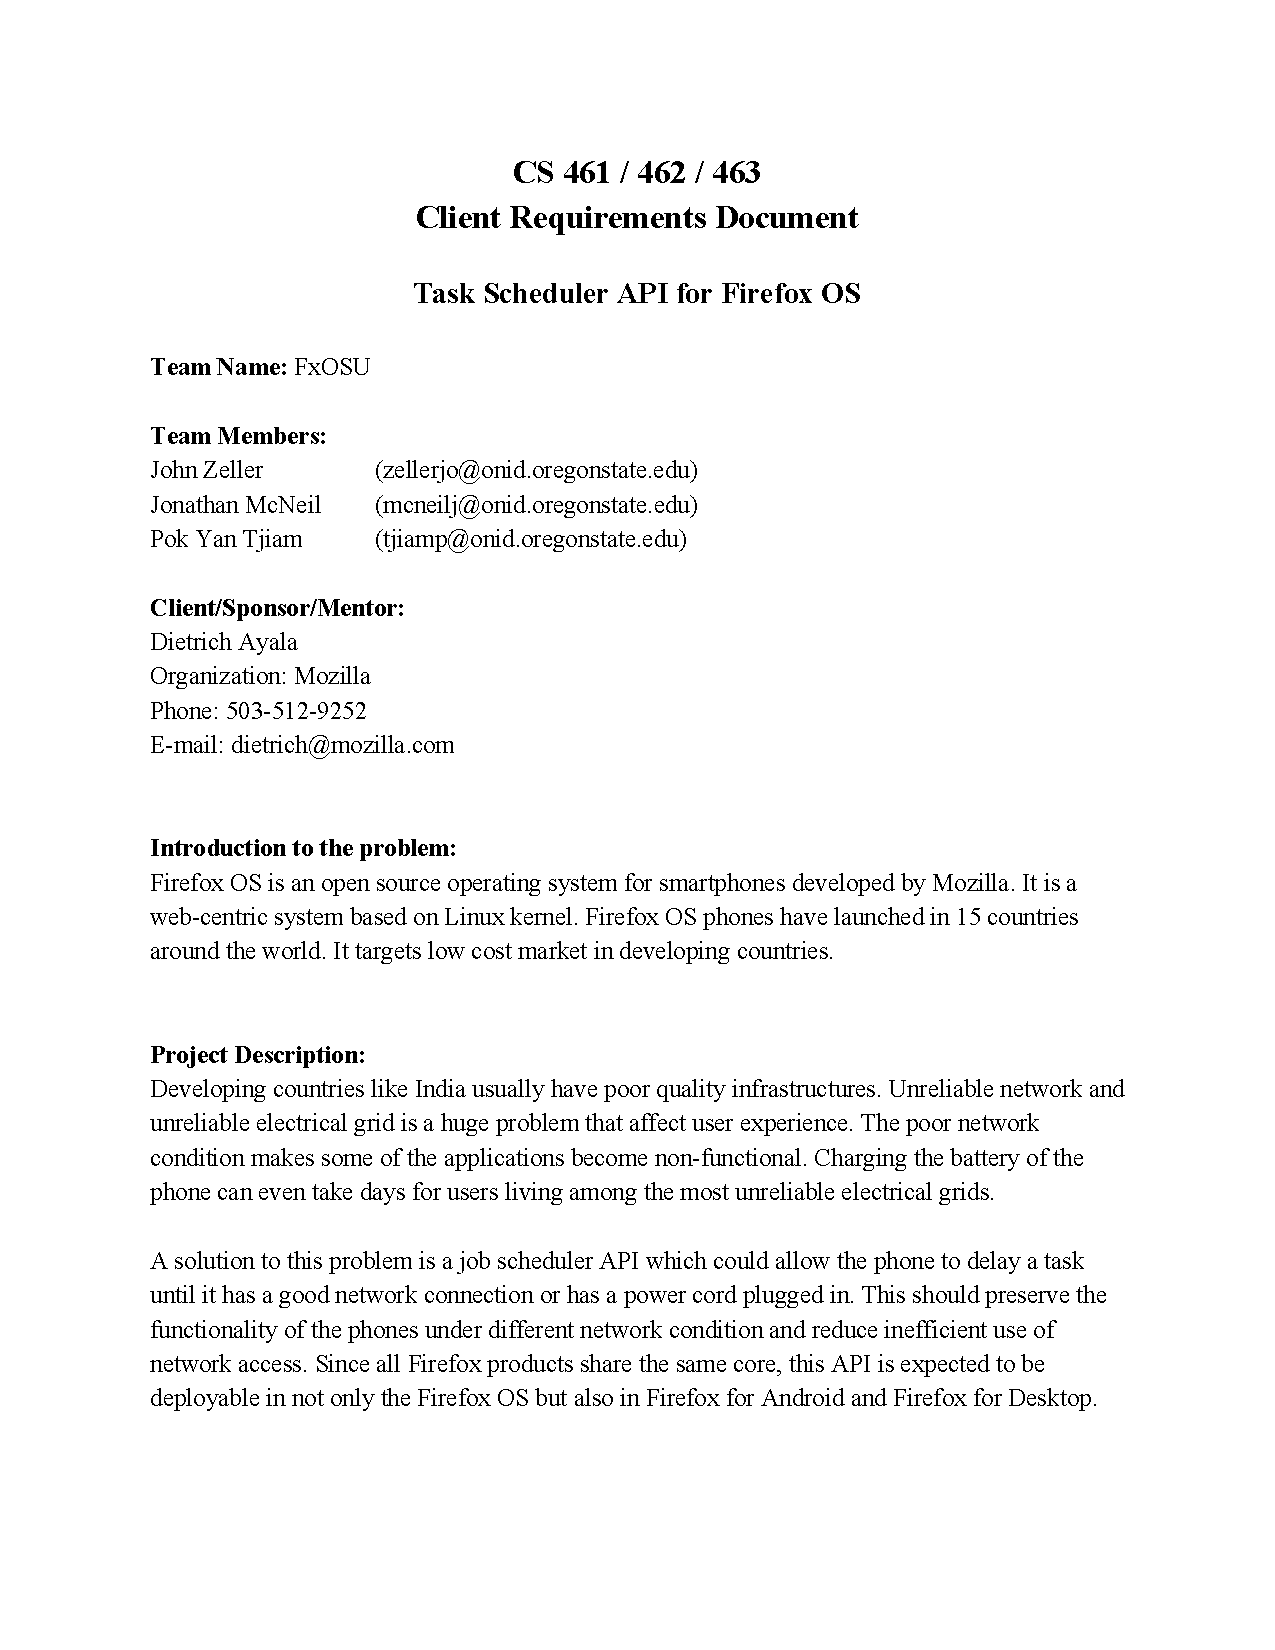
\includepdf[pages={1-8}]{images/requirementsdoc.pdf}

\subsection{Revisions}
% What new requirements were added? Why? 
% What existing requirements were changed? Why? 
% What existing requirements were deleted? Why? 
% Table featuring changed requirements
	% 1 | Requirement | What happened to it | Comments
% What was the final Gantt chart?

\subsubsection{Requirements}
As happens in most projects, requirements change, and ours was no different. Here are the changes that were made to our requirements and why.\\\\
\begin{tabular}{|l|l|l|l|}
\hline
\#  & Requirement 				& What Happened To It 		  & Comments \\ \hline
4	& The API should be written & Modified 					  & The reason for this... \\
	& in C++.					& Changed to "The API should  & \\
	&							& be written in C++ and/or	  & \\
	&							& JavaScript" 				  & \\ \hline
5 	& The API should be callable& Modified 					  & The reason for this... \\
	& by JavaScript executing in& First became "The API should& \\
	& the DOM in a web context. & be callable by JavaScript   & \\
	&							& executing in the window.",  & \\
	&							& Then modified again to 	  & \\
	&							& become "The prototype API   & \\
	&							& should be callable by 	  & \\
	&							& JavaScript executing in a   & \\
	&							& web sandbox." 			  & \\ \hline
6 	& The prototype API should  & Removed 				 	  & The reason for this... \\
	& be able to queue tasks. 	& New requirement was "The 	  & \\
	& 						 	& prototype API should be able& \\
	&							& be able to access data on   & \\
	&							& the battery level of the    & \\
	&							& device in order to determine& \\
	&							& if a task should be 		  & \\
	&							& executed." 				  & \\ \hline
7 	& The prototype API should  & Removed				 	  & The reason for this... \\
	& be able to prioritize		& New requirement was "The 	  & \\
	& tasks in the queue based	& protoype API should be able & \\
	& on network, battery and 	& to access data on the 	  & \\
	& system data.				& charging state of the device& \\
	&							& in order to determine if a  & \\
	&							& task should be executed."   & \\ \hline
\end{tabular}
\pagebreak

\begin{tabular}{|l|l|l|l|}
\hline
\#  & Requirement 				& What Happened To It 		  & Comments \\ \hline
8 	& The prototype API should	& Modified 					  & The reason for this... \\
	& be developer configurable,& Changed to "The prototype   & \\
	& to provide a force		& API should be developer 	  & \\
	& execution of a task after	& configurable, to provide a  & \\
	& a period of time.			& level of certainty about 	  & \\
	&							& network quality."			  & \\ \hline
9 	& The prototype API should  & Modified 				      & The reason for this... \\
	& be able to function  	   	& Changed to "The prototype   & \\
	& without error on Firefox  & API should be able to 	  & \\
	& OS, Firefox for Android,	& function without error on   & \\
	& and Firefox for Desktop.	& Firefox for Desktop."		  & \\ \hline
10 	& The API should be able to & Modified 				      & The reason for this... \\
	& access data on the quality& Changed to "The prototype   & \\ 
	& of the network in order to& API should be able to access& \\
	& determine if a task should& latency-related network     & \\
	& be executed.				& information to determine if & \\
	&							& a task should be executed." & \\ \hline
16 	& The API should be able to & Removed					  & The reason for this... \\
	& queue and postpone tasks	& New requirement was "The API& \\
	& from being dispatched.	& should be able to access 	  & \\
	&							& latency-related network 	  & \\
	&							& information to determine if & \\
	&							& a task should be executed." & \\ \hline
17 	& The API should be able to & Removed 					  & The reason for this... \\
	& prioritize queued tasks 	& New requirement was "The API& \\
	& based on accessible data  & should take into account the& \\
	& about the device and the  & type of network connection, & \\
	& environment.				& whether it be wifi, cellular& \\
	&							& data, etc."				  & \\ \hline
18	& The API should have a 	& Removed					  & The reason for this... \\
	& mechanism for dispatching & New requirement was "The API& \\
	& queued tasks.				& should be able to access 	  & \\
	&							& data about recent tx/rx 	  & \\
	&							& data."					  & \\ \hline
\end{tabular}
\pagebreak

\begin{tabular}{|l|l|l|l|}
\hline
\#  & Requirement 				& What Happened To It 		  & Comments \\ \hline
19 	& The API should be  	    & Modified 					  & The reason for this... \\
	& developer configurable, to& Changed to "The API should  & \\
	& prioritize application 	& be developer configurable,  & \\
	& specific tasks.			& to provide a level of 	  & \\
	&							& certainty about network 	  & \\
	&							& quality."					  & \\ \hline
20 	& The API should be  	    & Removed					  & The reason for this... \\
	& developer configurable,   & New requirement was "The 	  & \\
	& to provide a force  	    & prototype API should be able& \\
	& execution of a task after & to access data about recent & \\
	& a period of time.			& tx/rx data to determine if a& \\
	&							& task should be executed."	  & \\
	&							& Then, the requirement was   & \\
	&							& modified to become "The 	  & \\
	&							& prototype API should be able& \\
	&							& to see if the device has an & \\
	&							& internet connection to 	  & \\
	&							& determine if a task should  & \\
	&							& be executed."				  & \\ \hline
\end{tabular}
\pagebreak

\subsubsection{Gaant Chart}
Here is the final Gaant chart for how our project timeline actually turned out.

\begin{figure}[h!]
  \centering
	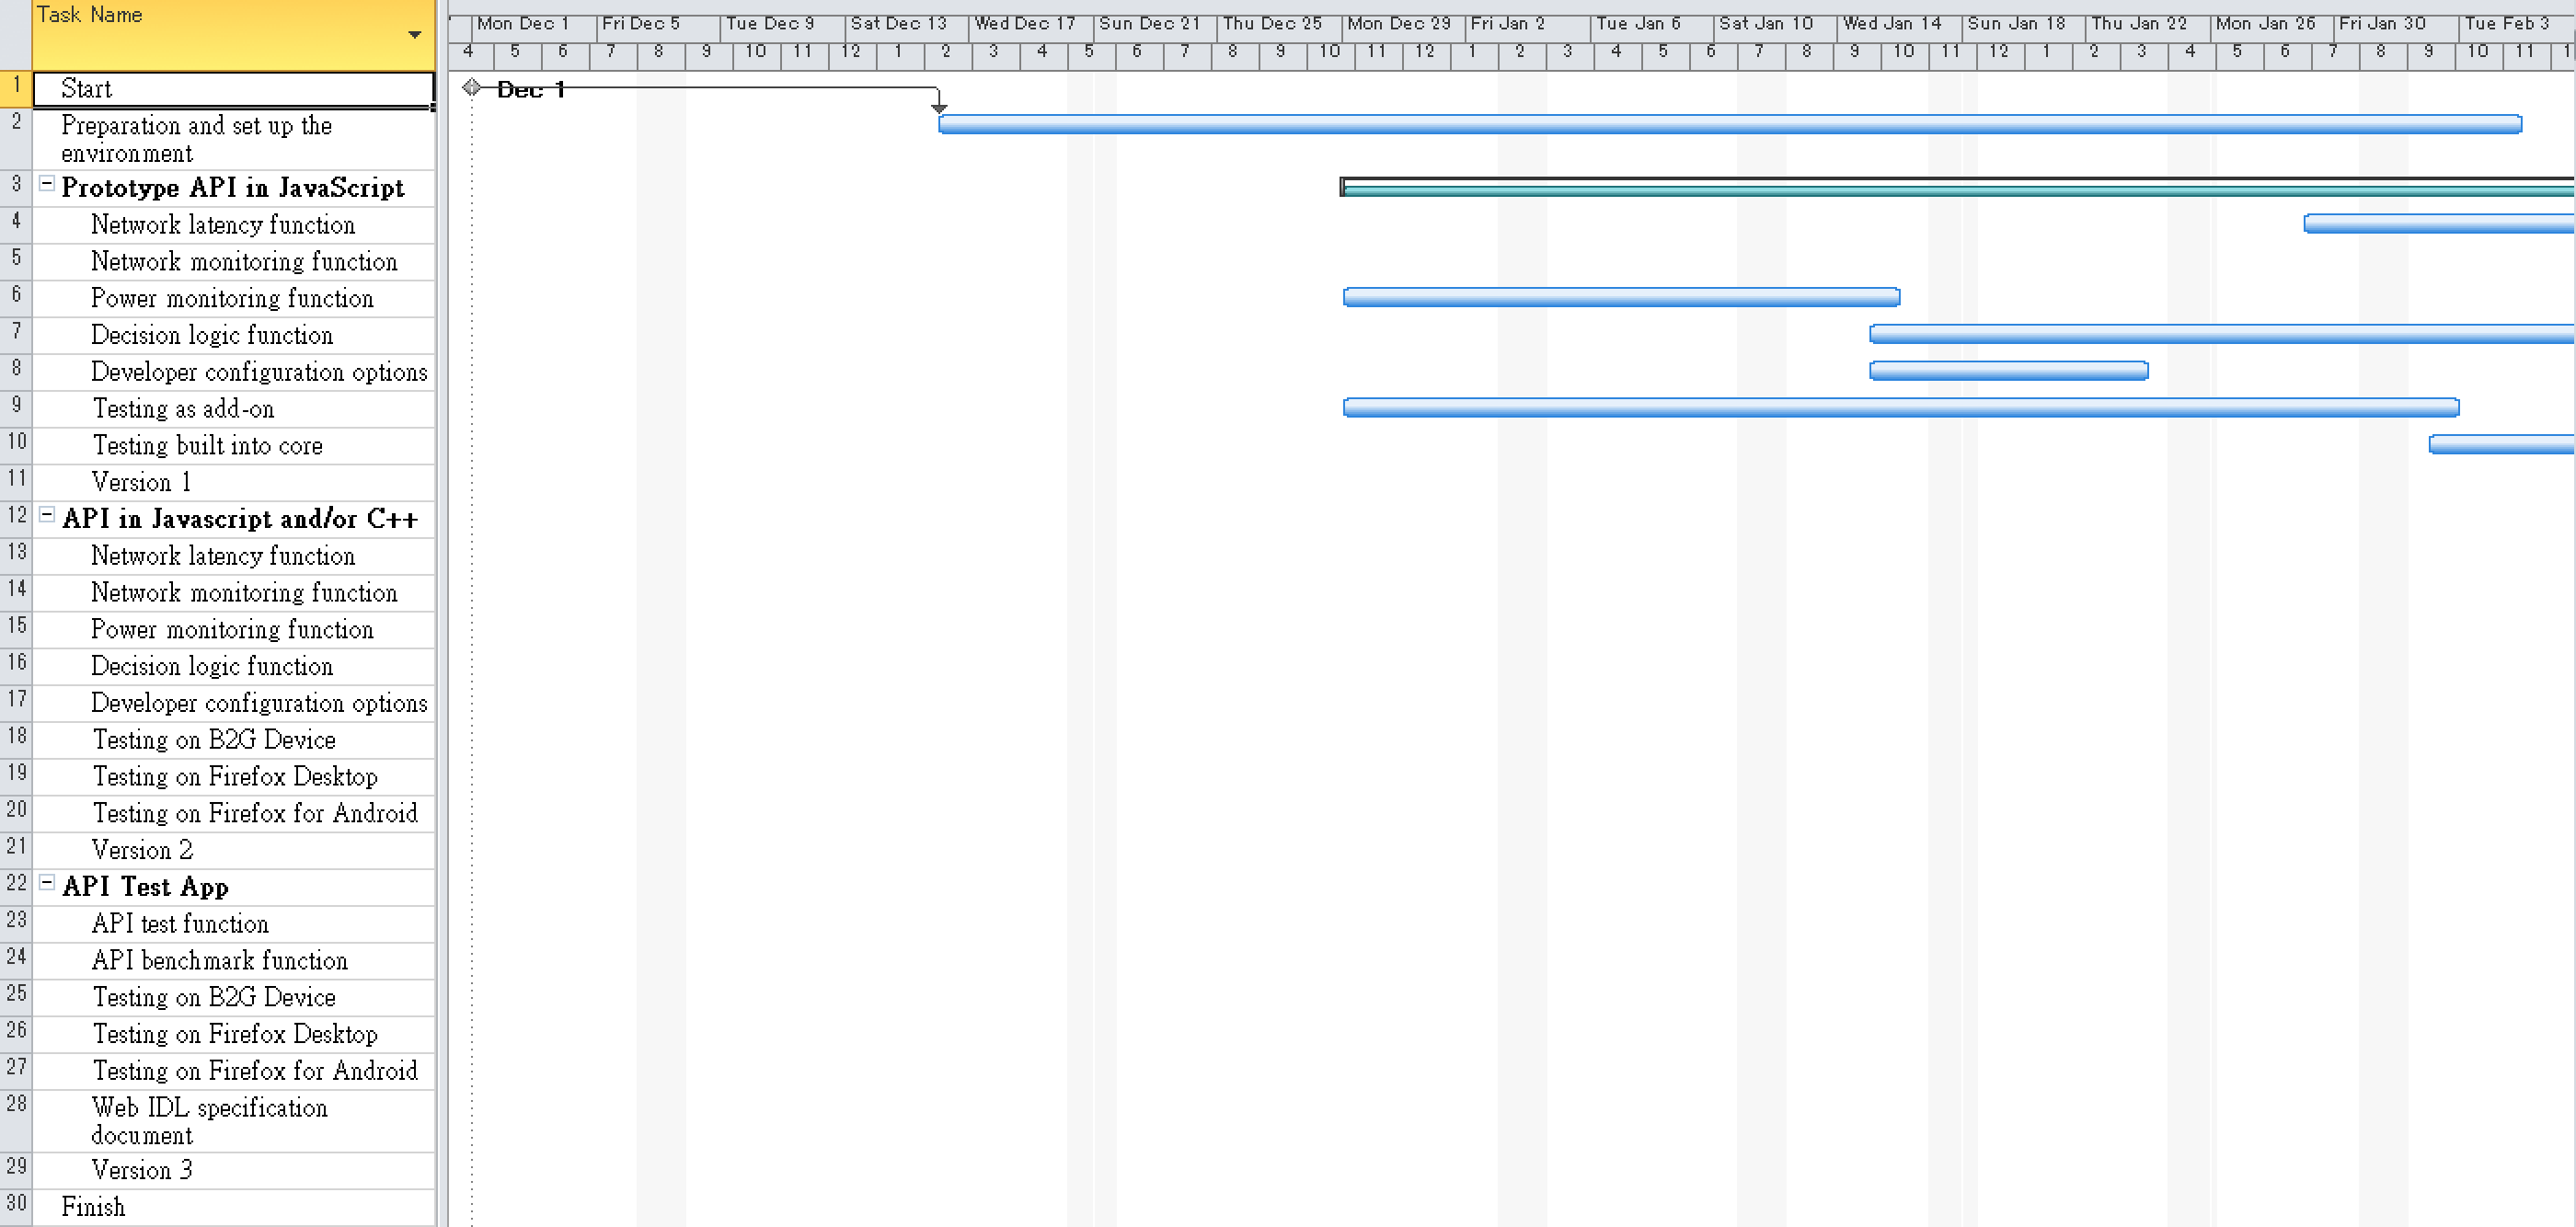
\includegraphics[scale=0.3]{finalgaant1.png}
  \caption{1 of 3: The final Gaant chart for how our project timeline actually turned out.}
\end{figure}
\begin{figure}[h!]
  \centering
	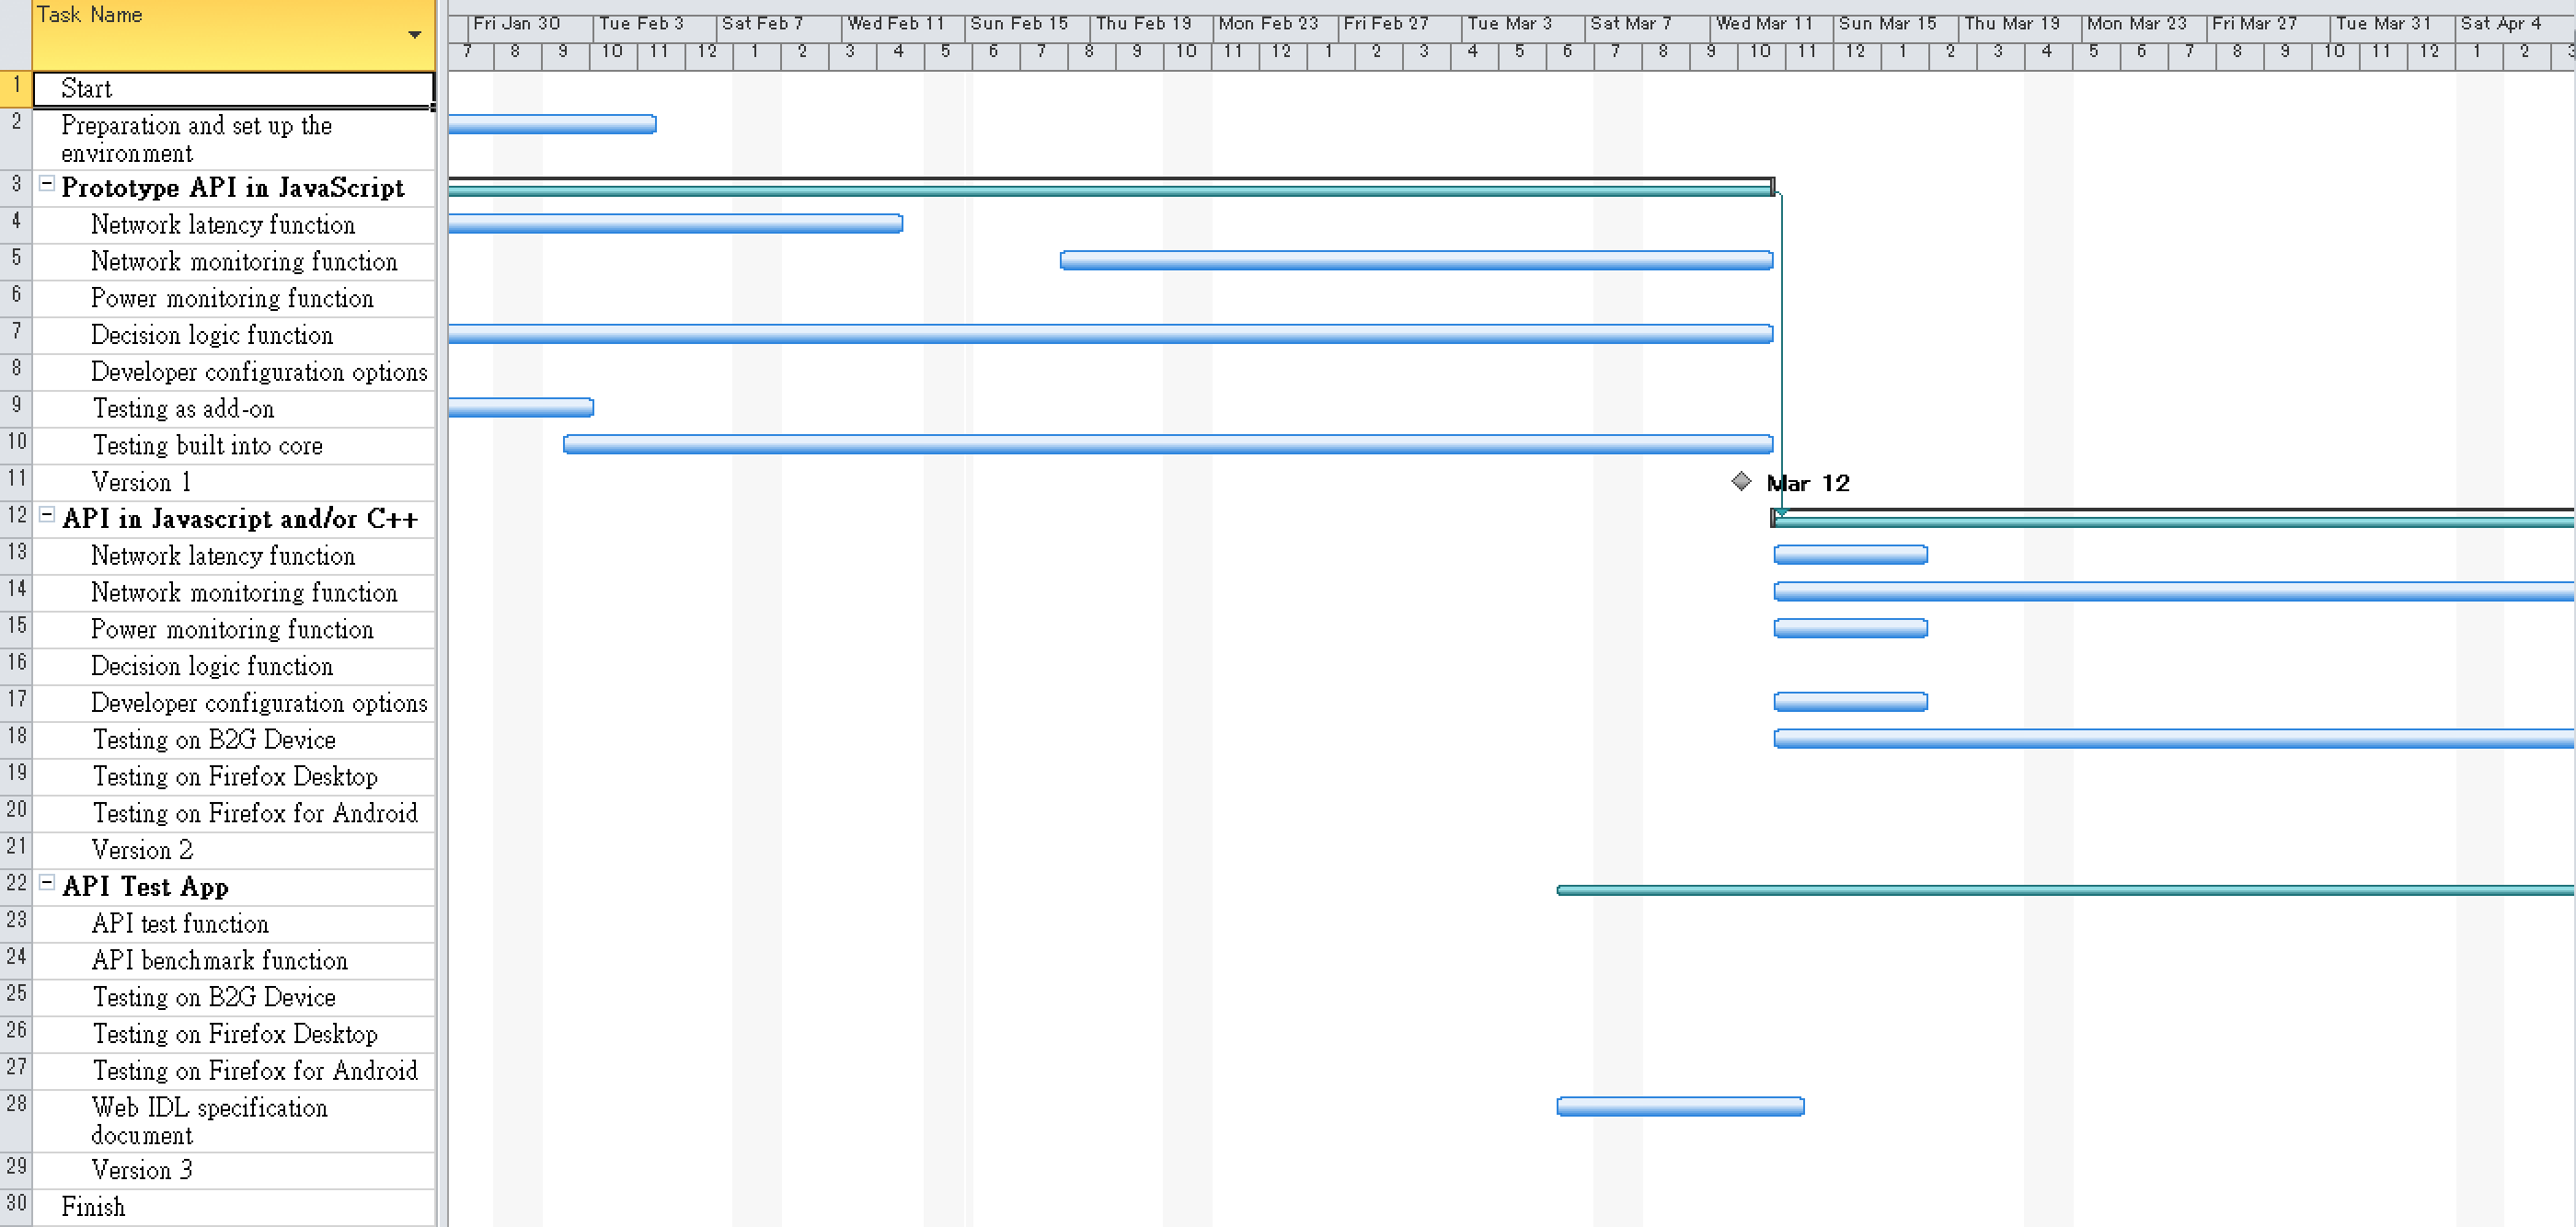
\includegraphics[scale=0.3]{finalgaant2.png}
  \caption{2 of 3: The final Gaant chart for how our project timeline actually turned out.}
\end{figure}
\pagebreak

\begin{figure}[h!]
  \centering
	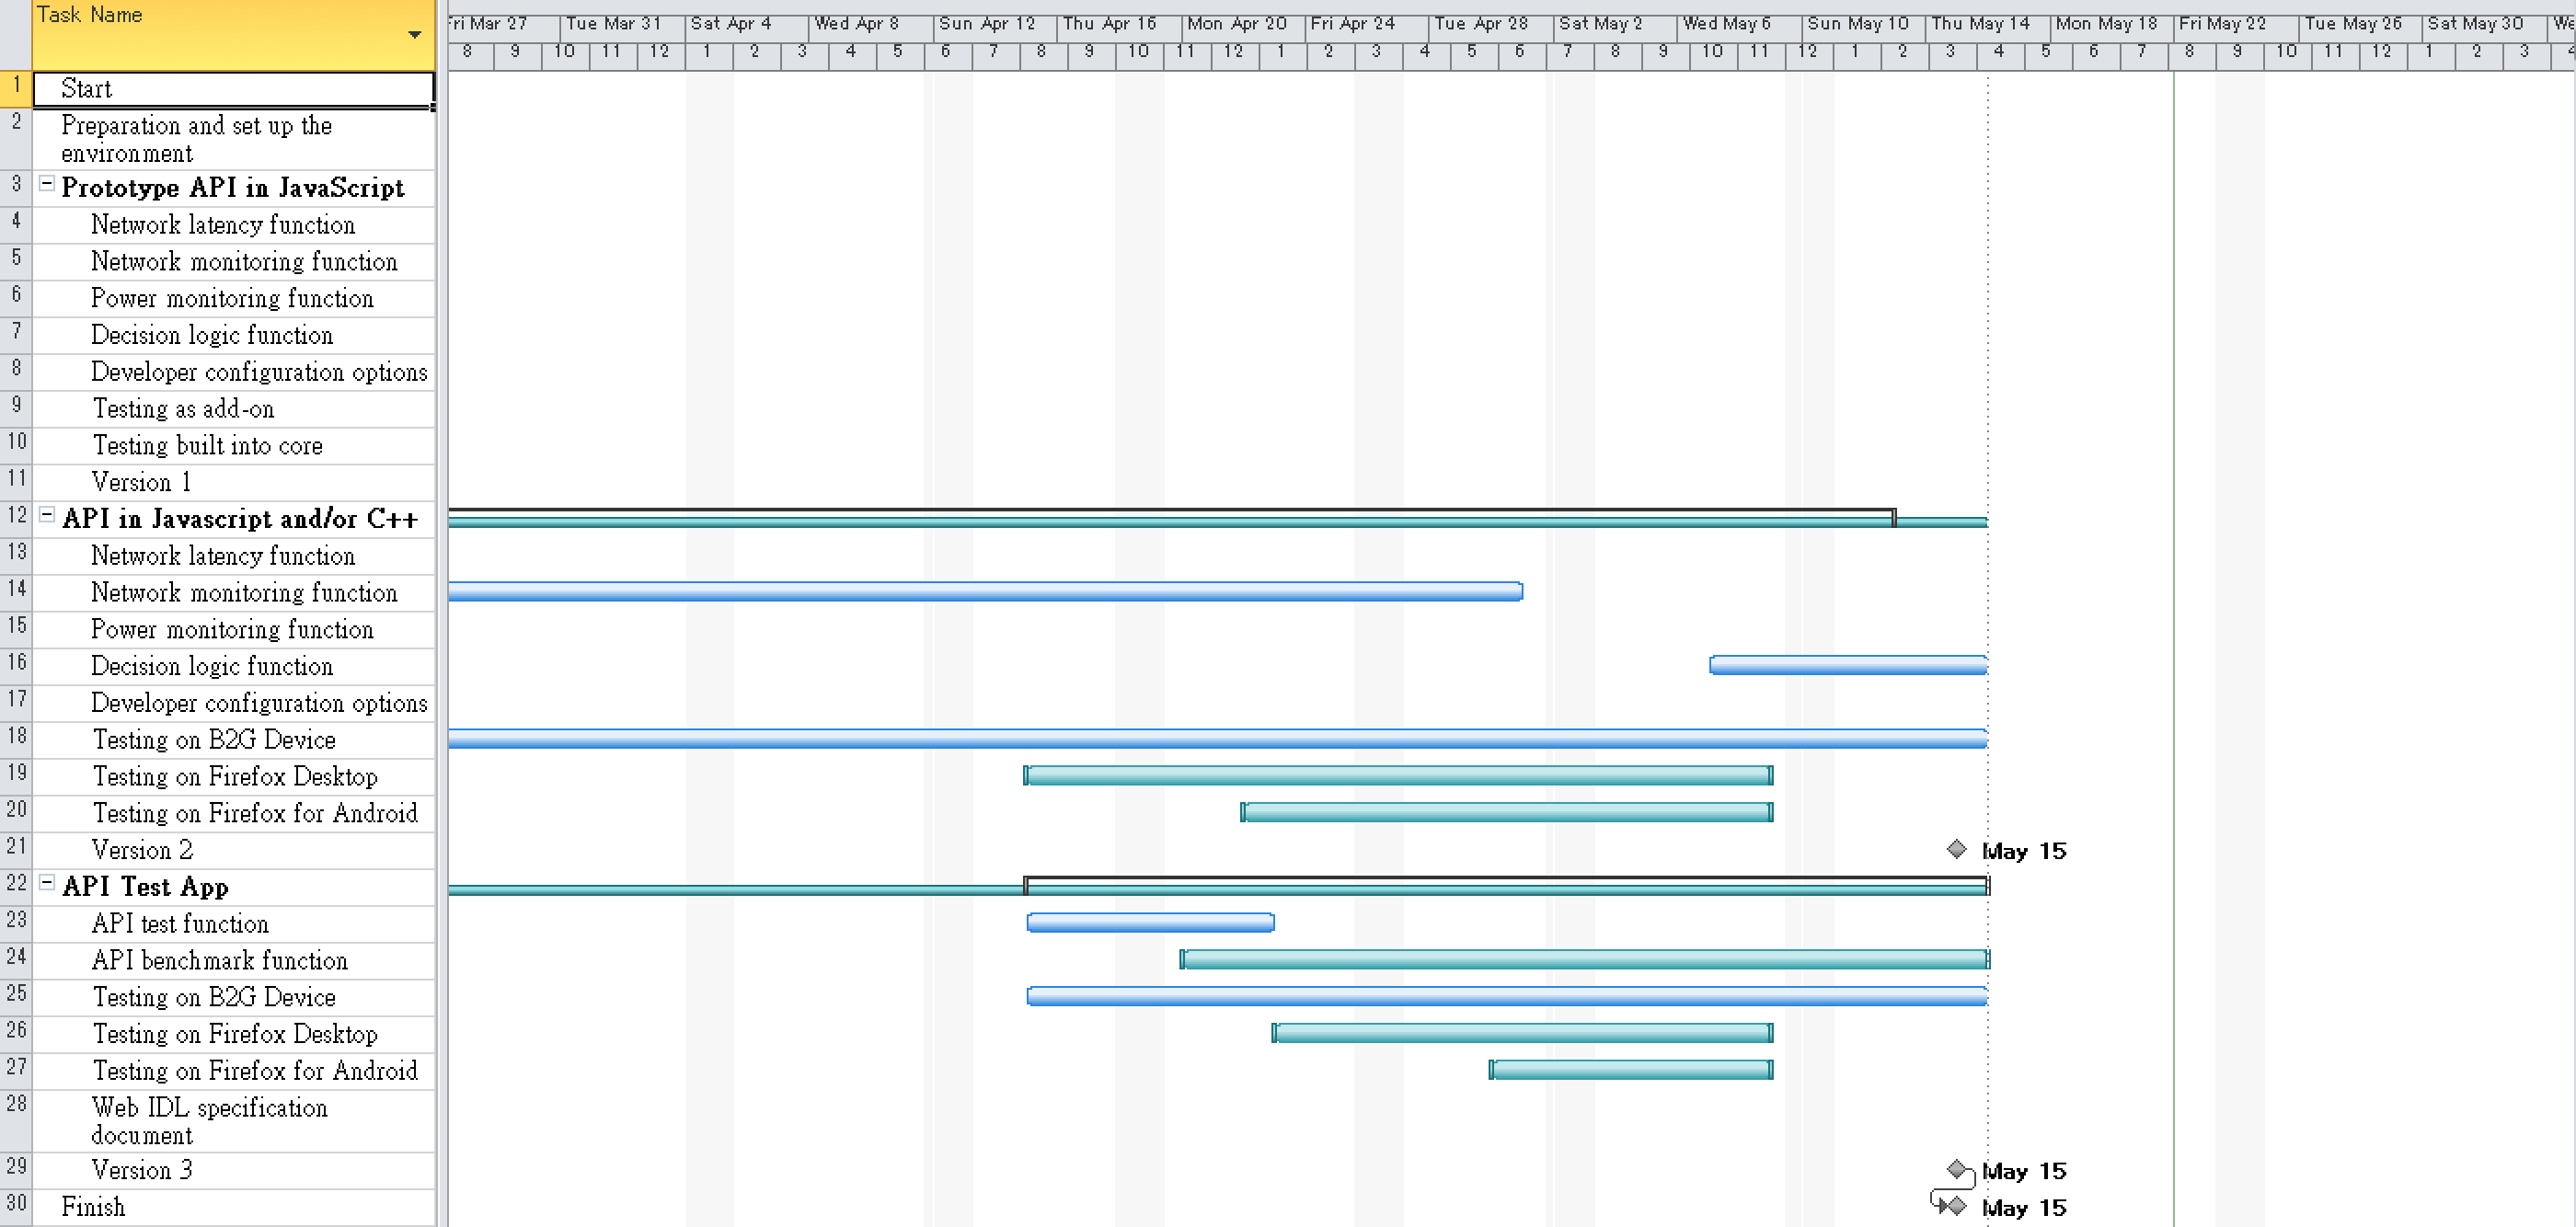
\includegraphics[scale=0.3]{finalgaant3.png}
  \caption{3 of 3: The final Gaant chart for how our project timeline actually turned out.}
\end{figure}
\pagebreak

\section{Weekly Team Blog Posts}
% These should be formatted nicely and clearly distinct from one another.
\subsection{Fall 2014}
\textbf{Week 5\\Friday, October 31, 2014\\}

\noindent Plans for coming week:
\begin{itemize}
\item Start working on the requirements document
\item Continues to research on Firefox OS
\end{itemize}

\noindent Progress since last week:
\begin{itemize}
\item Problem statement finished
\item Technology review finished
\item Project blog and project site set up
\item Problem statement and technology review uploaded to the project site
\end{itemize}

\noindent This week we set up our project blog and project site using Sharepoint space. The project site is used to store and share documents we made such as the problem statement and technology review to the whole team. The project blog is used to keep track of our progress on this project. We posted our progress updates on the project blog every week so that our client can know what we are currently working on. \\
\\
\textbf{Week 6\\Friday, November 7, 2014\\}

\noindent Plans for coming week:
\begin{itemize}
\item Continues to work on the requirements document
\item Continues research (necko), get familiar with Web IDL specifications
\end{itemize}

\noindent Progress since last week:
\begin{itemize}
\item Finished the basic structure of the requirements document
\end{itemize}

\noindent We expect to finish the introduction and project description parts of the requirements document, and think of some requirements for this project in the next week. We create our first draft of the requirement document in Word format instead of LaTeX because it is easier for us to edit it online. We stored our requirement document on Google Drive and shared it to the whole team as well as our client so that every one in our team can work on the document at the same time. Also, our client can give us immediate feedback without sending email but simply add a line somewhere on the document. We followed the format provided in the assignment page and finished the basic structure of the requirements document at the end of this week. \\
\\
\textbf{Week 7\\Friday, November 14, 2014\\}

\noindent Plans for coming week:
\begin{itemize}
\item Continues to work on the requirements document
\item Finish the requirment parts of the requirements document
\end{itemize}

\noindent Progress since last week:
\begin{itemize}
\item Finished the introduction part of the requirements document
\end{itemize}

\noindent We continue to work on the requirement document in this week. We combined the words FxOS and OSU to FxOSU and decided to use it as our team name. Our progress on the requirement document was pretty slow because we have to do more research on Firefox OS at the same time. At the end of this week we finished the introduction part of the requirements document and filled in some requirements of the project. \\
\\
\textbf{Week 8\\Friday, November 21, 2014\\}

\noindent Plans for coming week:
\begin{itemize}
\item Finish the whole requirements document
\item Get the requirements document signed
\item Start working at the poster
\end{itemize}

\noindent Progress since last week:
\begin{itemize}
\item Finished the project description part of the requirements document
\end{itemize}

\noindent This week we were still working on the requirement document. We were a bit behind schedule and need to finish the requirement document as soon as possible in order to get feedback from our client and get it signed before Thanksgiving. \\
\\
\textbf{Week 9\\Friday, November 28, 2014\\}

\noindent Plans for coming week:
\begin{itemize}
\item Finish the poster
\item Start working on the preliminary design document
\end{itemize}

\noindent Progress since last week:
\begin{itemize}
\item Requirements document finished and submited
\item Requirements document uploaded to the project site
\item Start working on the poster
\end{itemize}

\noindent Finally we finished the requirements document and got it signed. The requirements document was also uploaded to the project site. We felt like we have a problem on our time management. To prevent similar thing happens, we need to check each other's schedule and have more time to work together. \\
\\
\textbf{Week 10\\Friday, December 5, 2014\\}

\noindent Plans for coming week:
\begin{itemize}
\item Finish the preliminary design document
\item Finish the progress report
\item Meet with Professor McGrath for end-of-term meeting
\end{itemize}

\noindent Progress since last week:
\begin{itemize}
\item Preliminary Poster finished
\item Preliminary Poster uploaded to the project site
\end{itemize}

\noindent This week we started working on the poster that we will be using in the Expo and got it finished in this week. Since this is only a preliminary design of the poster, we did not fill in all the contents. The poster have a blue background and orange header and it follows the Firefox OS branding guidelines.
\\\\
Two of our team members, John and Jonathan, went to Portland to meet with our client and engineers from Mozilla. We have a more clear direction on what we are going to do. \\
\\
\textbf{Finals Week\\Friday, December 12, 2014\\}
Fall 2014, Finals week: \\
\\
\noindent Plans for the next term:
\begin{itemize}
\item working on the Javascript prototype
\item Research on Services Worker
\item Research on RequestSync
\end{itemize}

\noindent Progress since last week:
\begin{itemize}
\item Preliminary design document finished
\item Progress report finished
\end{itemize}

\noindent This term we spent most of the time working on documents and research. Next term we will start working on the prototype of our API and we will later move on to the implementation in C++.
\\\\
This week is the end of Fall term. The blog will stop updating until next term.

\subsection{Winter 2015}
\textbf{Week 1\\Friday, January 9, 2015\\}

\noindent Plans for coming week:
\begin{itemize}
\item Start working on the actual implementation
\end{itemize}

\noindent Progress since last week:
\begin{itemize}
\item Set up the weekly meeting with our TA
\item Set up our group meeting time
\item Requirements updated
\end{itemize}

\noindent Winter term begins and we get back to our project. In the first week, we scheduled a weekly meeting with our TA. and updated the requirements. We broke down our project into 24 requirements and each member handle 8 of them. We are expected to complete 6 requirements at the end of this term and 2 for the next term. \\
\\
\textbf{Week 2\\Friday, January 16, 2015\\}

\noindent Plans for coming week:
\begin{itemize}
\item Start working on the prototype API
\end{itemize}

\noindent Progress since last week:
\begin{itemize}
\item Updated requirements approved
\item Requirements completion list submitted
\end{itemize}

\noindent This week we got our new requirements approved and divided works to each member. We also started our implementation of prototype API using JavaScript. \\
\\
\textbf{Week 3\\Friday, January 23, 2015\\}

\noindent Plans for coming week:
\begin{itemize}
\item working on the prototype API
\end{itemize}

\noindent Progress since last week:
\begin{itemize}
\item Updated requirements approved
\end{itemize}

\noindent Again we update one of the requirement to make it more specific and got it approved. After speaking with our sponsor, we decided to implement our prototype API as a Firefox addon instead of putting it into the Firefox core, while the  C++ API will still need to be put into the core. \\
\\
\textbf{Week 4\\Friday, January 30, 2015\\}

\noindent Plans for coming week:
\begin{itemize}
\item Finish the implementation of the prototype API
\item Finish the first 9 requirements and get ready for demo
\end{itemize}

\noindent Progress since last week:
\begin{itemize}
\item Created a draft of the prototype API
\end{itemize}

\noindent This week we were working on the prototype API. Because our API will communicate between C++ and Javascript, we implement our prototype API as a XPCOM component. We succesfully installed the prototype API as an addon to the Firefox but we failed to call the C++ function in JavaScript. We will keep working on it and try to make the addon works in the next week. \\
\\
\textbf{Week 5\\Friday, February 6, 2015\\}

\noindent Plans for coming week:
\begin{itemize}
\item Finish the implementation of the prototype API
\item Test the prototype API on desktop, Android and Firefox OS
\item Demo the prototype API to the TA
\end{itemize}

\noindent Progress since last week:
\begin{itemize}
\item Implemented the prototype API addon using addon SDK
\item Battery level, device charging state and network latency data are accessible from the prototype API
\end{itemize}

\noindent This week we were still working on the prototype API. Since the addon-via-manifest prototype API does not works well, we tried another method and implemented the addon via SDK. Also, it turns out that some of the functionality of our API are only available on the Firefox OS but not the desktop version. Therefore we need to write a new prototype for the Firefox OS device. \\
\\
\textbf{Week 6\\Friday, February 13, 2015\\}

\noindent Plans for coming week:
\begin{itemize}
\item Start working on the actual API using C++ or Javascript
\end{itemize}

\noindent Progress since last week:
\begin{itemize}
\item Prototype API finished
\item Completed the demo of first 9 requirements to the TA
\end{itemize}

\noindent This week we finally finished the prototype API. The prototype can detect the battery level, charging state of the device, network connection type and shows latency-related information. We also changed our requirements after talking to the sponsor to scope the prototype down so that we have more time to focus on the actual API. \\
\\
\textbf{Week 7\\Friday, February 20, 2015\\}

\noindent Plans for coming week:
\begin{itemize}
\item Continue working on the actual API using C++ or Javascript
\end{itemize}

\noindent Progress since last week:
\begin{itemize}
\item Start working on the actual API using C++ or Javascript
\end{itemize}

\noindent This week we keep on working on the API. A few weeks before we got a developer reference phone called Flame from our sponsor. We began testing our API on this Firefox OS device to make sure our API works on all platform of Firefox. \\
\\
\textbf{Week 8\\Friday, February 27, 2015\\}

\noindent Plans for coming week:
\begin{itemize}
\item Continue working on the API using C++ or Javascript
\end{itemize}

\noindent Progress since last week:
\begin{itemize}
\item Continue working on the API using C++ or JavaScript
\end{itemize}

\noindent This week we are still working on the API. Most of the functions of the actual API are same as the prototype API. Some of the new functions of the actual API include collect network status information, access system load information and to integrate with existing API such as ServiceWorker and RequestSync. Each of our group member take charge of one of these function. \\
\\
\textbf{Week 9\\Friday, March 6, 2015\\}

\noindent Plans for coming week:
\begin{itemize}
\item Finish the next 9 requirements
\item Finish the implementation of the API
\end{itemize}

\noindent Progress since last week:
\begin{itemize}
\item Continue working on the implementation of the API
\end{itemize}

\noindent We are going to demo the next 9 requirements to the TA in the final week. We hope to finish the implementation of our API next week and test it before we demo. \\
\\
\textbf{Week 10\\Friday, March 13, 2015\\}

\noindent Plans for coming week:
\begin{itemize}
\item Finish the next 9 requirements
\item Finish the implementation of the API
\item Demo the 9 requirements to the TA
\end{itemize}

\noindent Progress since last week:
\begin{itemize}
\item poster updated
\item Continue working on the implementation of the API
\end{itemize}

\noindent This week we updated the poster and keep working on the API. We are going to demo the requirements next week but some of the requirement are still incomplete. Some of the functions of our API took longer than we expected to implemented. \\
\\
\textbf{Finals Week\\Friday, March 20, 2015\\}
Winter 2015, Finals week: \\
\\
\noindent Plans of the next term:
\begin{itemize}
\item Finish the implementation of the API
\item Prepare for Expo
\end{itemize}

\noindent Progress since last week:
\begin{itemize}
\item Finished the demo of winter term requirements
\end{itemize}

\noindent This term we finished most of the implementation of the API.  We tested our API mainly on Firefox desktop. In the next term we will focus on the implementation and testing of our API on Firefox OS.

\subsection{Spring 2015}
\textbf{Week 1\\Friday, April 3, 2015\\}

\noindent Plans for coming week:
\begin{itemize}
\item Continue to work on the FxOSUService API
\end{itemize}

\noindent Progress since last week:
\begin{itemize}
\item Set up the weekly meeting with our TA
\end{itemize}

\noindent Spring term begins. This week we scheduled a weekly meeting with our TA. We have to complete the last 6 requirements before the Expo and prepare for the Expo onMay 15th. \\
\\
\textbf{Week 2\\Friday, April 10, 2015\\}

\noindent Plans for coming week:
\begin{itemize}
\item Continue to work on the FxOSUService API
\end{itemize}

\noindent Progress since last week:
\begin{itemize}
\item Met with our sponsor via video call
\end{itemize}

\noindent This week we had a meeting with our sponsor. We keep on working on our API and hope to finish it quickly so that we have time to work on the test app. \\
\\
\textbf{Week 3\\Friday, April 17, 2015\\}

\noindent Plans for coming week:
\begin{itemize}
\item Continue working on the FxOSUService API
\item working on the test app
\end{itemize}

\noindent Progress since last week:
\begin{itemize}
\item Updated the poster
\end{itemize}

\noindent This week we are still working on the requirements. We also start working on a test app that benchmark the performance of our API. The test app is implemented in Javascript. We also updated our poster. \\
\\
\textbf{Week 4\\Friday, April 24, 2015\\}

\noindent Plans for coming week:
\begin{itemize}
\item Continue working on the FxOSUService API
\item Continue working on the test app
\item Update the poster
\end{itemize}

\noindent Progress since last week:
\begin{itemize}
\item Modify the format of our poster
\end{itemize}

\noindent This week we need to modify the poster to a specified format. It won't be hard because we only need to change the layout and content can stay the same. We need to finish our poster before May 1st. We are also working on the final draft of our API and hope to get it done by next week. \\
\\
\textbf{Week 5\\Friday, May 1, 2015\\}

\noindent Plans for coming week:
\begin{itemize}
\item Finish the test app
\item Demo the requirements to our TA
\end{itemize}

\noindent Progress since last week:
\begin{itemize}
\item Finished the poster
\item Finished our API
\end{itemize}

\noindent This week we finished the poster. The final draft of our FxOSUService API is finished and is working. Expo is approaching. We are going to demo our requirements to the TA and prepare for the Expo after the demo. \\
\\
\textbf{Week 6\\Friday, May 8, 2015\\}

\noindent Plans for coming week:
\begin{itemize}
\item Prepare for the Expo
\end{itemize}

\noindent Progress since last week:
\begin{itemize}
\item Finished all the requirements
\item Finished the test app
\item Finished the demo
\end{itemize}

\noindent This week we finished the test app and finished the demo of our requirements. Expo is next Friday and we have to start prepare for it. \\
\\
\textbf{Week 7\\Friday, May 15, 2015\\}

\noindent Plans for coming week:
\begin{itemize}
\item Start working on the report and presentation
\end{itemize}

\noindent Progress since last week:
\begin{itemize}
\item Expo is over
\end{itemize}

Expo is over. 

\pagebreak

\section{Project Poster}
This is the final project poster that we used when demoing our project at the Engineering Expo.

\includepdf[pages={1},angle=90]{images/poster.pdf}


\section{Project Documentation}
% How does your project work?
% 	What is its structure?
% 	What is its Theory of Operation?
% 	Block and flow diagrams are good here. 
% How does one install your software, if any?
% How does one run it?
% Are there any special hardware, OS, or runtime requirements to run your software?
% Any user guides, API documentation, etc.
\subsection{Overview}
Our project took shape through 4 distinct phases: Research, Prototype, Implementation, and Test App. Our research phase took us through understanding fundamental Firefox paradigms like XPCOM and foundational concepts like IPC, JavaScript Runtime, and WebIDL. Our research phase stayed active throughout most of our Prototype and Implementation phases, as we learned new concepts that were necessary for us to accomplish the design we'd set out to build. When building our prototype, we learned a lot about what has to be built into the core of Firefox, as opposed to being tested in a priveleged JavaScript add-on. Implementation brought a lot of its' own challanges, smoothed over by the things learned during prototyping. And finally, our test app helped to highlight the strengths and weaknesses of the final implementation that we had come up with.
\pagebreak

\subsection{Structure}
There are almost 4 million lines of code in Firefox, and our project barely scratches that surface. Here is the breakdown of the source code effected by our work.

\begin{figure}[h!]
  \centering
		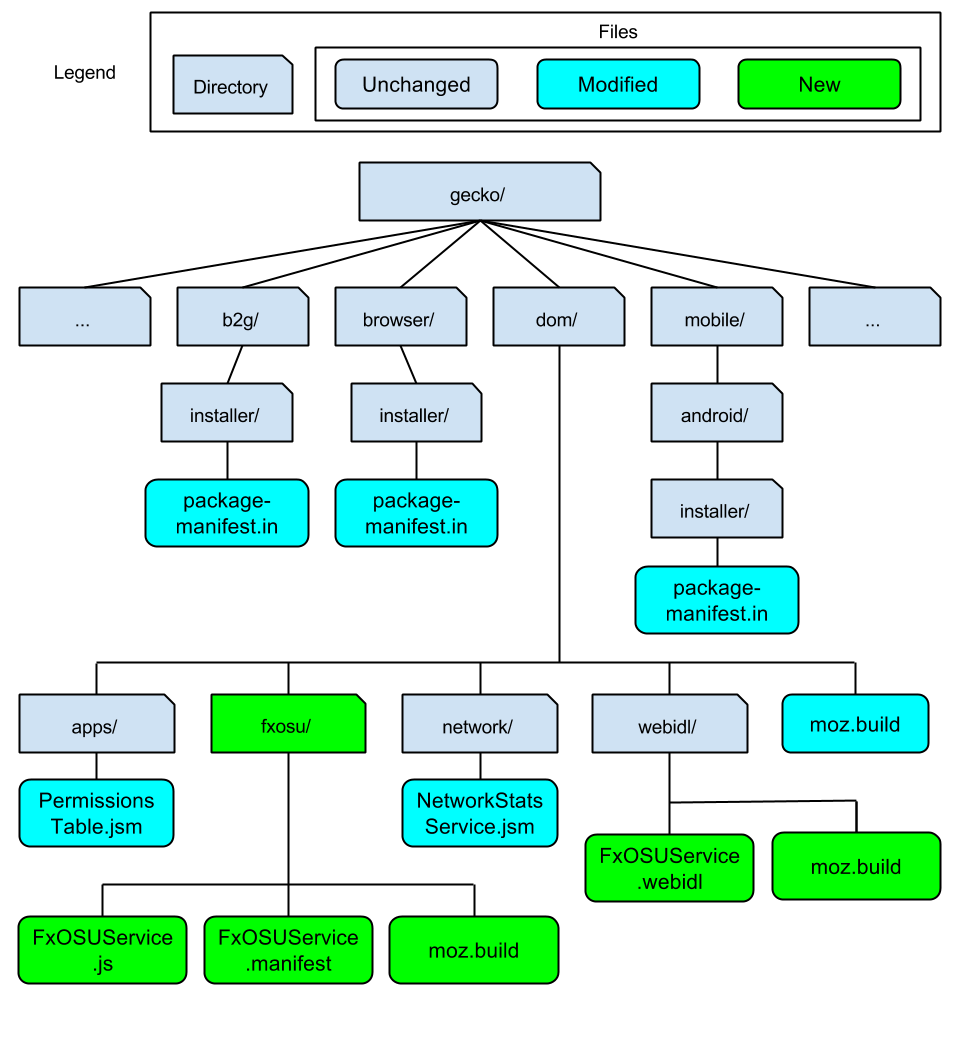
\includegraphics[scale=0.4]{codestructure.png}
  \caption{Files and directories effected by our project.}
\end{figure}
\pagebreak

\subsection{Building/Running from Source}

\subsection{API Documentation}

\pagebreak

\section{Learning New Technology}
% What web sites were helpful? (Listed in order of helpfulness.)
% What, if any, reference books really helped?
% Were there any people on campus that were really helpful? 
There were a number of websites that were helpful during the course of researching, designing, implementing and testing our project. Here is a list of the websites that we found most useful, organized from most to least helpful:
\begin{enumerate}
	\item Mozilla Developer Network (\href{https://developer.mozilla.org/en-US/}{https://developer.mozilla.org/en-US/})
	\item Mozilla Wiki (\href{https://wiki.mozilla.org/}{https://wiki.mozilla.org/})
	\item Boot2Gecko Mailing List (\href{https://groups.google.com/forum/\#!forum/mozilla.dev.b2g}{https://groups.google.com/forum/\#!forum/mozilla.dev.b2g})
	\item Gaia Mailing List (\href{https://groups.google.com/forum/\#!forum/mozilla.dev.gaia}{https://groups.google.com/forum/\#!forum/mozilla.dev.gaia})
	\item StackOverflow (\href{http://stackoverflow.com/}{http://stackoverflow.com/})
\end{enumerate}

\noindent Other resources that we found really helpful included:
\begin{enumerate}
	\item IRC (irc.mozilla.org)
		\subitem Find more info here: \href{https://wiki.mozilla.org/IRC}{https://wiki.mozilla.org/IRC}
\end{enumerate}
\pagebreak

\section{What did we learn from all of this?}
\subsection{John Zeller}
\textbf{What technical information did you learn?}\\
I learned a lot about JavaScript. When I first began working on this project, I came in with the urge to do and learn something outside of my comfort zone. I usually write in Python, and have primarily used Python in the 3 internships that I have had. So, writing JavaScript, and moreover, becoming aquanted with Firefox source code were both amazing learning experiences.
\\\\
Digging into the Firefox source code gave me a much better idea of how a browser is put together. Understanding the complexities of a relatively small part of Firefox, such as IPC, has given me a great insight into the complexity of this code base.
\\\\
\textbf{What non-technical information did you learn?}\\
I learned more about the organization of teams within Mozilla, and the separation of efforts in one product, accross multiple teams. There really is a huge amount of institutional knowledge, and a lot of it has been written out in their wiki pages. I also learned that a lot of those wiki pages are out of date, and need some love.
\\\\
\textbf{What have you learned about project work?}\\
I learned a lot about the importance of a design cycle such as Agile. Most of the senior design process is sort of intrinsically setup in a Waterfall design cycle, but you are free to iterate on that, running your own weekly, bi-weekly, monthly etc. Agile cycles. Our group in particular ran into this pretty hard, and we ended up changing 10 of our 24 requirements. When we originally wrote our requirements document during Fall term, we had an idea of what the project would look like, and not 4 weeks later, that idea changed significantly.
\\\\
\textbf{What have you learned about project management?}\\
Other than the importance of design cycles, as I mentioned above, I learned about the importance of constant communication with your project customer. It's very possible that the ideas you have begun to spin within your own mind, and in the hive mind of the project group, could be wildly different, or even slightly misaligned from that of the project customer, and the much larger hive mind of your customers organization.
\\\\
\textbf{What have you learned about working in teams?}\\
I've certainly learned about the importance of communication throughout the project. Often we would run into issues where one or more of our group members were lost, while perhaps at least one knew the way forward. Clear communication and clearing up questions is something that produces a well oiled machine.
\\\\
\textbf{If you could do it all over, what would you do differently?}\\
If I could do it all over again, I would spend significantly more time researching our project during October, before our requirements document was written. If we were able to have overcome many of the changes that we needed to make later on, this would have seriously increased the ease of implementation that we experienced throughout the project.
\\

\subsection{Pok Yan Tjiam}
\textbf{What technical information did you learn?}\\
\\\\
\textbf{What non-technical information did you learn?}\\
\\\\
\textbf{What have you learned about project work?}\\
\\\\
\textbf{What have you learned about project management?}\\
\\\\
\textbf{What have you learned about working in teams?}\\
\\\\
\textbf{If you could do it all over, what would you do differently?}\\
\\

\subsection{Jonathan McNeil}
\textbf{What technical information did you learn?}\\
\\\\
\textbf{What non-technical information did you learn?}\\
\\\\
\textbf{What have you learned about project work?}\\
\\\\
\textbf{What have you learned about project management?}\\
\\\\
\textbf{What have you learned about working in teams?}\\
\\\\
\textbf{If you could do it all over, what would you do differently?}\\
\pagebreak

\section{Appendix I}
% Essential Code Listings. You don't have to include absolutely everything, but if someone wants to understand your project, there should be enough here to learn from. If you worked within a larger project, something like a patch file might be a good way to go.
Code
\pagebreak

\section{Appendix II}
% Anything else you want to include. Photos, etc.

\end{document}